\documentclass[8pt]{beamer}

\usepackage[utf8]{inputenc}
\usepackage{default}
\usepackage{hyperref}
\usepackage{textpos}
\usepackage{verbatimbox}
%\usepackage{animate}
\usepackage{graphicx}
\usepackage{multimedia}
\usepackage{pdfpages}
\usetheme{Copenhagen}

\title{Blockchains}
\subtitle{Cryptocurrencies and Consortium Blockchains}
\author{Tero Keski-Valkama, Elisa Patronen}
\institute{
\includegraphics[height=1.4cm]{CybercomG_logo_Classic_RGB.png}}
\date{2017-02-05}

\addtobeamertemplate{frametitle}{}{%
\begin{textblock*}{100mm}(10.95cm,-0.8cm)

\includegraphics[height=0.8cm]{cybercom-blue.png}
\end{textblock*}}


\begin{document}

\frame{\titlepage}
 
\begin{frame}
\frametitle{What is Blockchain}

\begin{itemize}
 \item Blockchain is a collection of cryptotechnologies to achieve a distributed consensus about immutable, additive data in an untrusted environment.
 \begin{enumerate}
  \item Blockchain is a sequence of records, or blocks, so that each block contains a hash digest of the previous block (which recursively contains the hash digest of the previous block and so on).
  \item A consensus mechanism with rules to determine which blocks are accepted to be the next block in the blockchain. Many solutions such as proof-of-work, proof-of-stake, proof-of-burn,
        Practical Byzantine Fault Tolerance, and hybrids.
  \item A discovery and broadcast infrastructure to relay transactions and blocks to peers and miners.
  \item Application-specific public key or other cryptography to prove identities of parties in transactions, wallets and so on.
  \item Microcode used to define the transaction semantics or smart contracts, such as \href{https://en.bitcoin.it/wiki/Script}{\textcolor{blue}{Bitcoin Script}},
        \href{http://solidity.readthedocs.io/en/latest/}{\textcolor{blue}{Solidity}}
        or \href{https://github.com/IBM-Blockchain/learn-chaincode}{\textcolor{blue}{Chaincode}}.
 \end{enumerate}
 \item In blockchain, a single valid block can be used to validate the whole chain of blocks to deep history so that anyone can make sure that nothing has been altered in the stored data,
       by checking that the hashes of the previous block always matches the content of the previous block.
 \item The consensus mechanism offers guarantees that all parties have a converging view in the blockchain regarding what is valid and what is not. It prevents changing the history and
       that the whole blockchain integrity is guaranteed.
\end{itemize}

\end{frame}

\begin{frame}
\frametitle{There Shall Be No Blockchain But Bitcoin}

\begin{figure}[tb]
 \centering
  \movie[width=10cm,height=7.5cm,autostart]{click}{./blockchain_images/Blockchain-visualisoinnit-kuva1.mp4}
\end{figure}

\end{frame}

\begin{frame}
\frametitle{Example of a Consortium Blockchain: Hyperledger Architecture}

\begin{figure}[tb]
 \centering
 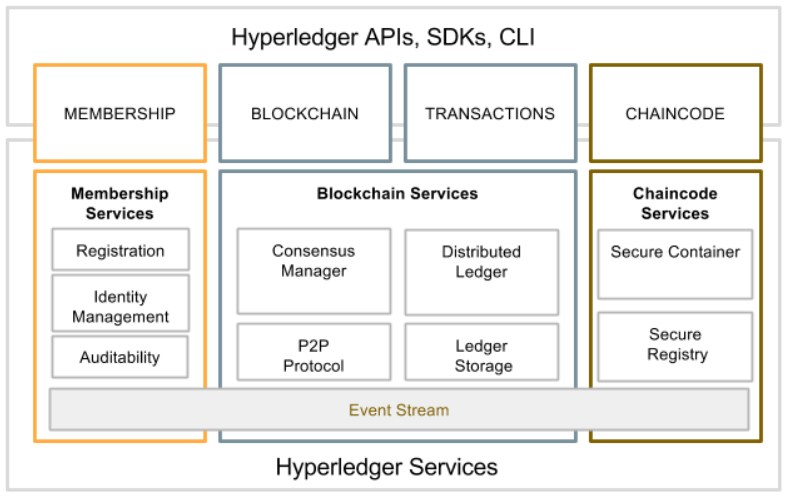
\includegraphics[width=6 cm,keepaspectratio=true]{./blockchain_images/hyperledger_architecture.png}
 \caption{Hyperledger Architecture}
\end{figure}

\end{frame}

\begin{frame}
\frametitle{Comparison of Associated Technologies}

\begin{tabular}{| l | c | c | c |}
\hline
 & \shortstack{Distributed \\ Database} & \shortstack{Consortium \\ Blockchain} & \shortstack{Cryptocurrency \\ Blockchain} \\
\hline
\shortstack{Consensus \\ mechanism} & \shortstack{Simple \\ parallel consistency} & \shortstack{Byzantine \\ Fault Tolerance} & \shortstack{Proof-of-Work, \\ Proof-of-Stake, \\ or a hybrid} \\
\hline
\shortstack{Requires \\ a cryptocurrency} & no & no & yes \\
\hline
\shortstack{Access} & Closed & Controlled & Open \\
\hline
\shortstack{Peers} & None & Validated & Untrusted \\
\hline
\end{tabular} 

\end{frame}

{
\setbeamercolor{background canvas}{bg=}
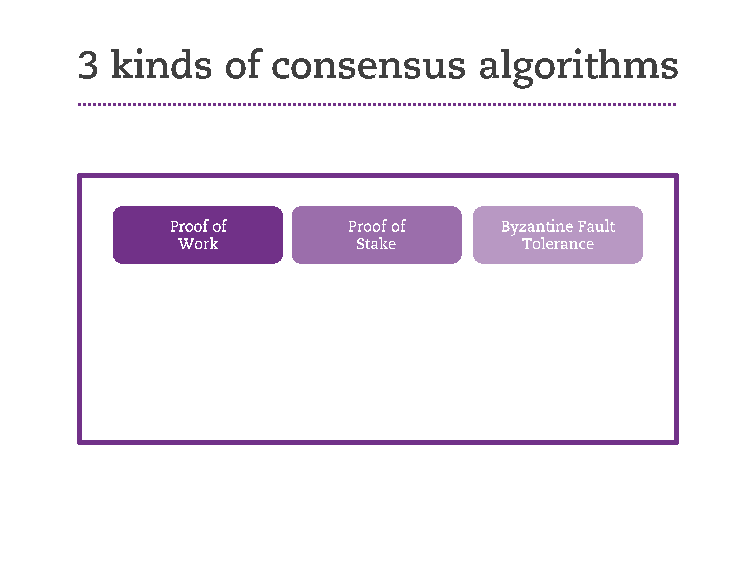
\includepdf[pages=1-5]{./blockchain_images/Blockchain-visualisoinnit2.pdf}
}

\begin{frame}
\frametitle{Consensus Mechanisms – Starting from Bitcoin}

\begin{columns}
\begin{column}{0.9\textwidth}

\begin{itemize}
 \item Consensus is inherently a game theoretic concept in Byzantine systems, because the peers can try to cheat.
 \item In open ecosystems it must be made economically infeasible to break the rules or the goals of the system. This leads to the requirement of having a cryptocurrency built into the system.
       In practice, a validating peer gains cryptocurrency for processing transactions, and this cryptocurrency only has value if the whole system works.
 \item The Bitcoin network can process the maximum of 7 transactions per second with the current block size limit of 1 MB.
 \item Calculating Bitcoin mining hashes requires about 1 W of power for 1 GH/s of computation for the most energy efficient ASIC implementations.
 \item The current hashrate of the Bitcoin network of 3,051,683,778 GH/s translates to a power of about 3 GW.
 \item In standard reindeers of 200 kg, this amounts to burning 2.25 reindeers of equivalent coal every second.
 \item In closed consortiums, it is feasible to get rid of peers behaving incorrectly, so expensive proof-operations can be avoided.
\end{itemize}
\end{column}
\begin{column}{0.1\textwidth}
% For Adobe Reader
%%\animategraphics[autoplay,loop,width=1cm]{10}{blockchain_images/porot-}{0}{9}
% For Linux Okular

\movie[width=1cm,height=5cm,autostart]{click}{./blockchain_images/porot.mp4}
\end{column}
\end{columns}
\end{frame}

{
\setbeamercolor{background canvas}{bg=}
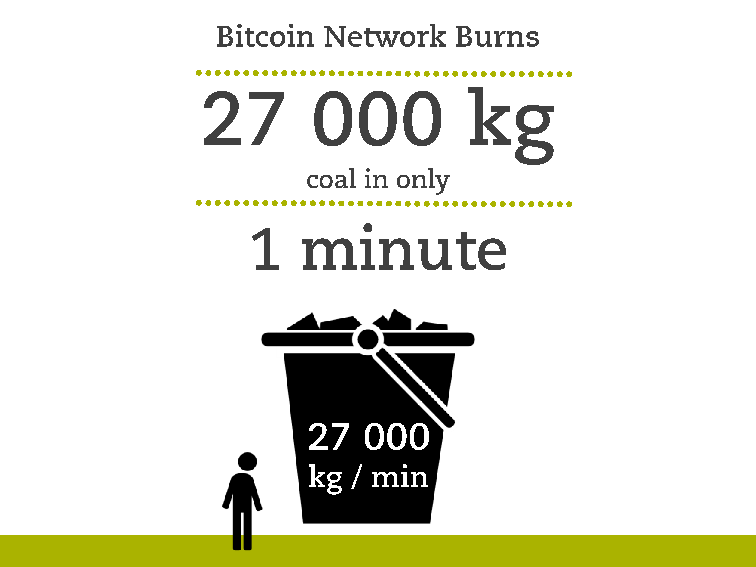
\includepdf[pages=1-3]{./blockchain_images/Blockchain-visualisoinnit-valas.pdf}
}

\begin{frame}
\frametitle{Proof of Work – Bitcoin, Litecoin, Dogecoin, etc.}

\begin{itemize}
 \item The point of Proof-of-Work is to prove that you have spent real resources in generating the block.
 \item Proof-of-work algorithms include for example Bitcoin double SHA256, or Dogecoin/Litecoin Scrypt.
 \item Bitcoin includes a double SHA-256 hash of the block in the blocks, and the block is only accepted if the hash value is lower than the difficulty limit. Hence, block hashes start with lots of zeros, for example:
       0x0000000000000000012fdce7dd73fddb087e66f4f6bb9672667b854282855669 for the block 
       \href{https://blockexplorer.com/block/0000000000000000012fdce7dd73fddb087e66f4f6bb9672667b854282855669}{\textcolor{blue}{\#451676}}
 \item Bitcoin Proof-of-Work does not require a lot of memory and can be easily implemented as an ASIC chip $ \rightarrow $ all miners are based on cheap ASICs now, and the hashrate is basically limited by energy costs.
       These ASICs are special-purpose machines and cannot be used for any other purpose than mining Bitcoins.
 \item Litecoin and several other coins use Scrypt algoritm as Proof-of-Work. This algorithm requires more memory (128 kB to match a typical CPU L2 cache), and memory is difficult to implement on an ASIC.
       Litecoin and Dogecoin can be mined with general purpose GPUs and even CPUs, and even in browsers. This has an effect of moving the bottleneck towards more expensive, but ubiquitous general purpose hardware
       from simple energy use.
\end{itemize}
\end{frame}

\begin{frame}
\frametitle{Proof of Stake – Ether after 2017, Peercoin}

\begin{itemize}
 \item Proof-of-Stake is a proposed alternative to energy wasting Proof-of-Work. Instead of proving you have done work, you prove you own a number of coins.
 \item Generally, for each block each coin gets a random chance of determining the next block.
 \item In 2017, Ethereum (Ether) moves to Proof-of-Stake algorithm, Casper. Some cryptocurrencies use a hybrid between Proof-of-Work and Proof-of-Stake.
 \item Game theoretic worries: If the miners have no stake, why would they play fair?
\end{itemize}
 \centering
 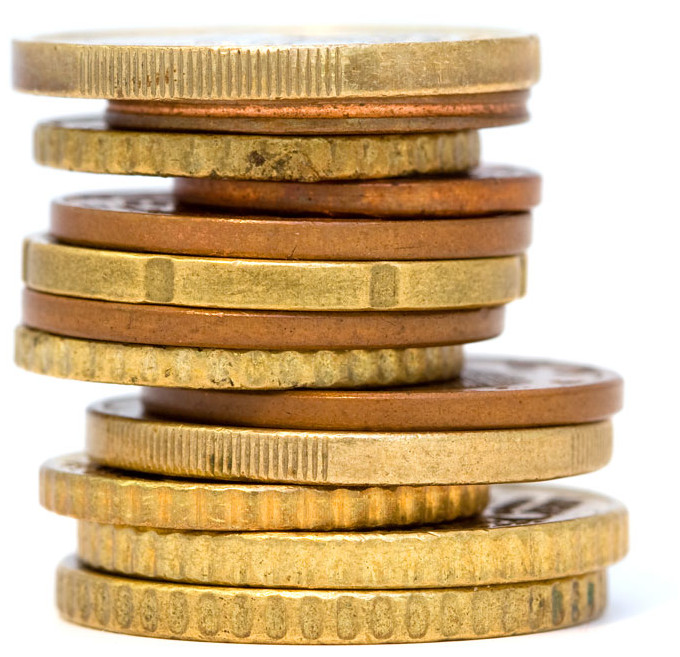
\includegraphics[width=4.5 cm,keepaspectratio=true]{./blockchain_images/coins.jpg}

\end{frame}

\begin{frame}
\frametitle{Byzantine Fault Tolerance}
\begin{itemize}
 \item Byzantine Fault Tolerance refers to a general game theoretic mathematical problem where distributed parties try to achieve consensus in spite of unreliable messaging and hostile actors.
 \item There are several algorithms and implementations with different characteristics.
 \item Practical Byzantine Fault Tolerance algorithm useful for consortium blockchains, but cannot be used for open blockchains.
 \item Byzantine Fault Tolerance algorithms do not generally consider an open system where new actors can join at will, and therefore they implicitly assume a kind of a Proof-of-Stake through association to the group.
 \item These algorithms generally need a centralized identity management to prevent a Sybil attack. Although it could be said that the centralized identity manager could freely perform a Sybil attack in these systems.
\end{itemize}
 \centering
 
\includegraphics[width=3 cm,keepaspectratio=true]{./blockchain_images/friends.jpg}
\end{frame}

\begin{frame}
\frametitle{Inside Blockchain}

\begin{figure}[tb]
 \centering
 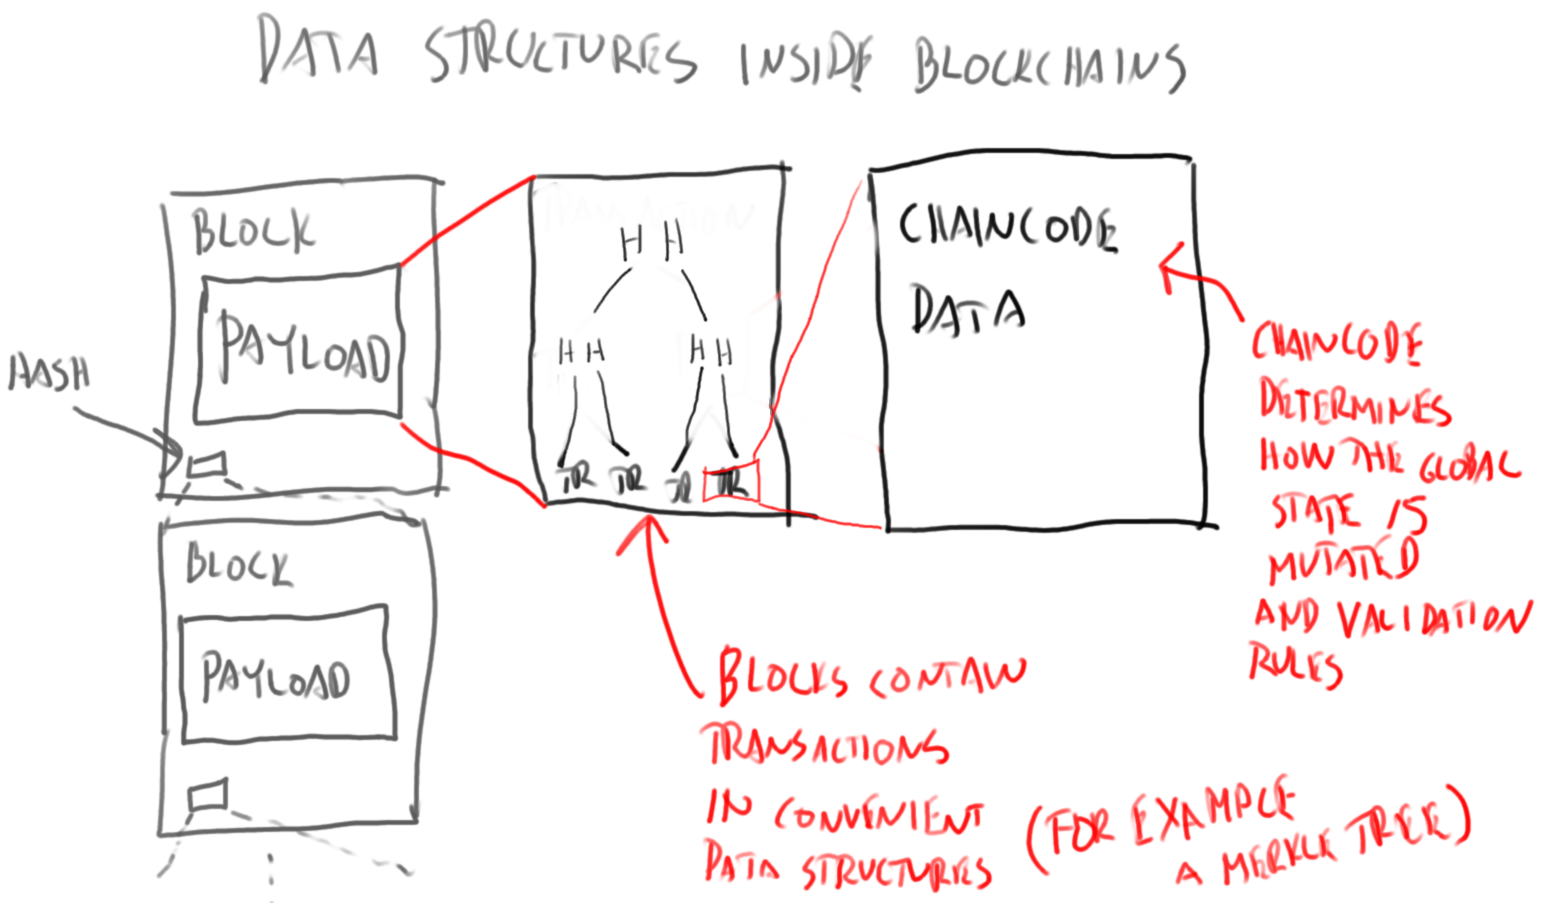
\includegraphics[width=8 cm,keepaspectratio=true]{./blockchain_images/inside_blockchains.png}
 \caption{Inside Blockchain}
\end{figure}

\end{frame}

\begin{frame}
\frametitle{Inside Bitcoin Transactions}

\begin{figure}[tb]
 \centering
 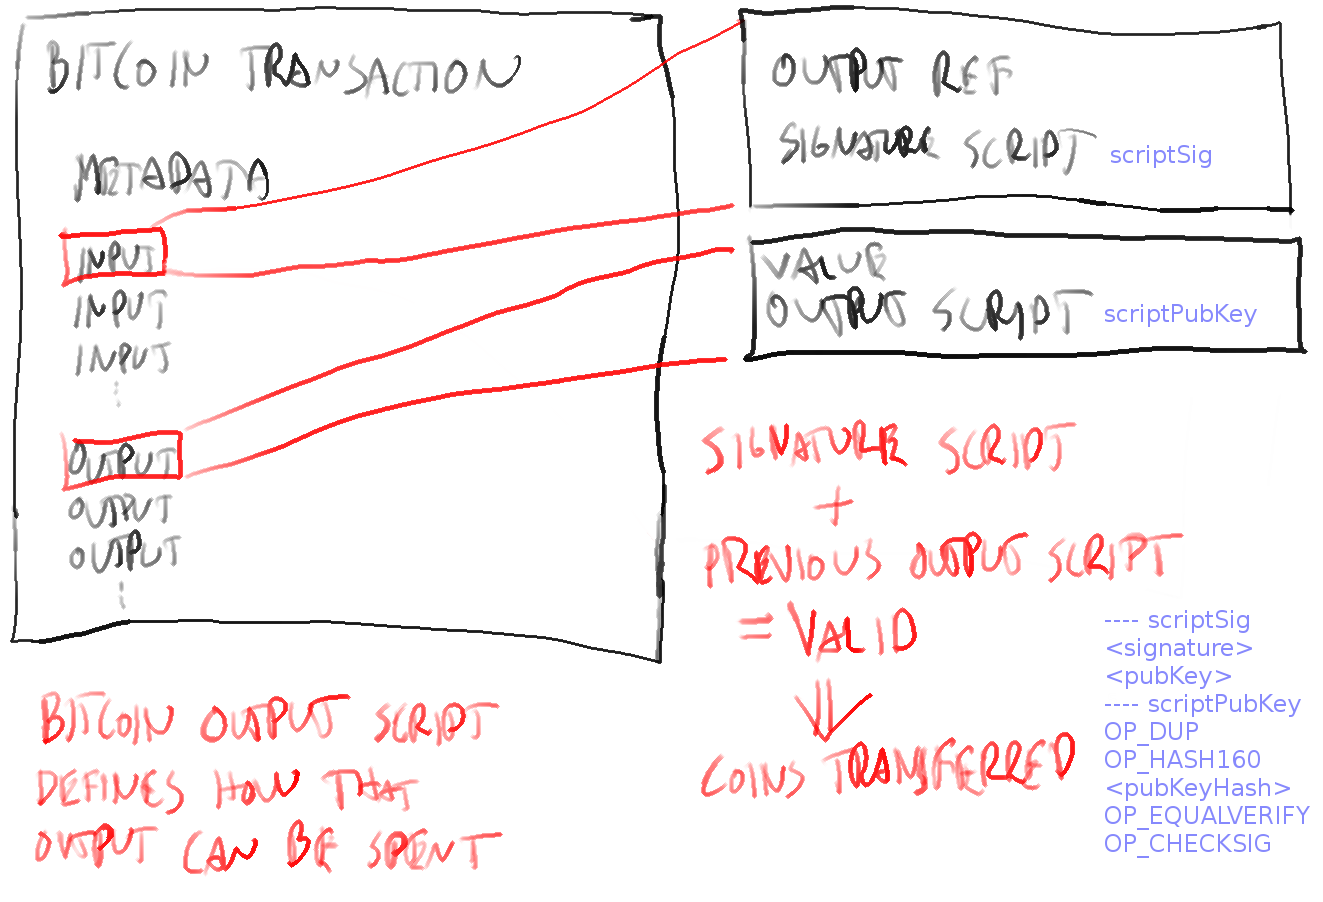
\includegraphics[width=10 cm,keepaspectratio=true]{./blockchain_images/bitcoin_transactions.png}
 \caption{Inside Bitcoin Transactions}
\end{figure}

\end{frame}

\begin{frame}
\frametitle{Comparison of Chaincode Languages}

\begin{columns}
\begin{column}{0.5\textwidth}
Constrained
\begin{itemize}
 \item Bitcoin Script
 \item Allow complex transactions (e.g. multisig), but no smart contracts or general purpose computing.
 \item The execution time is limited to a specific maximum per transaction.
 \item A special transaction set limits the utility of the blockchain to a specific application.
\end{itemize}
\end{column}
\begin{column}{0.5\textwidth}
Turing Complete
\begin{itemize}
 \item Hyperledger Chaincode, Ethereum Solidity
 \item Allow smart contracts and general purpose computing. Even \href{https://en.wikipedia.org/wiki/Synereo}{\textcolor{blue}{``world computer''}}.
 \item Requires either transaction gas, a closed set of trusted peers, or whitelisted (non-Turing complete) transaction patterns.
\end{itemize}
\end{column}
\end{columns}

\end{frame}

{
\setbeamercolor{background canvas}{bg=}
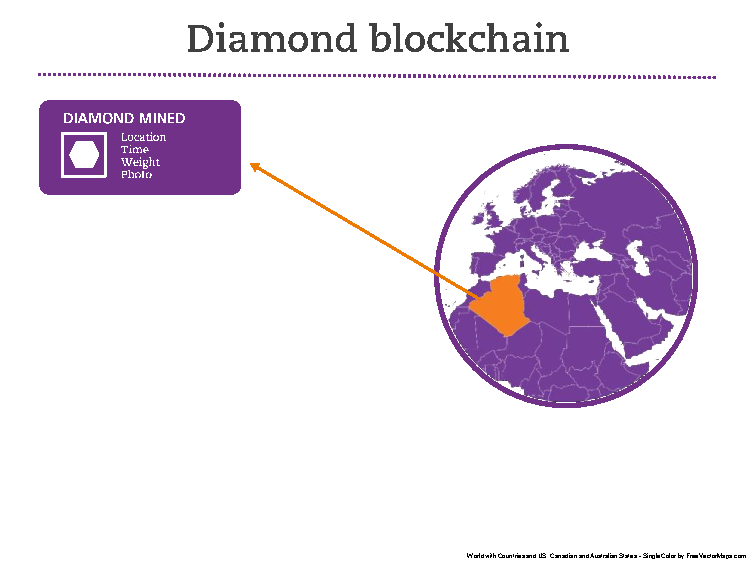
\includepdf[pages=1-8]{./blockchain_images/Blockchain-visualisoinnit5-diamond.pdf}
}

\begin{frame}
\frametitle{Guardtime KSI}
\begin{itemize}
 \item Estonian Guardtime offers a timestamp-hashing service based on Hash Calendar, which is a special type of a Merkle tree.
 \item Linked timestamping ties specific signing events together with time so that they cannot be altered without invalidating the whole chain.
 \item The service can be used to sign any data hash to irrevocably tie it to a specific time.
 \item The signature can then be used to prove that the hashed document existed at a claimed time.
 \item Applications include for example:
 \begin{itemize}
   \item tamper-proofing logs, as a tampered log entry would not have a valid timestamp signature, as it did not exist at the claimed time.
   \item Providing proof that a specific event happened at a certain point of time (not later than a given time).
 \end{itemize}
 \item The infrastructure is secured by using periodical hash calendar roots published through widely witnessed media such as Financial Times and Twitter.
\begin{figure}[tb]
 \centering
 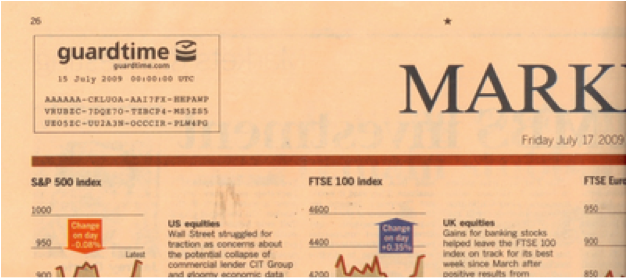
\includegraphics[width=3 cm,keepaspectratio=true]{./blockchain_images/widely_witnessed_media.png}
\end{figure}
\end{itemize}

\end{frame}

\begin{frame}
\frametitle{Links}
\begin{itemize}
 \item \href{https://d28rh4a8wq0iu5.cloudfront.net/bitcointech/readings/princeton\_bitcoin\_book.pdf?a=1}{\textcolor{blue}{Princeton course book: Bitcoin and Cryptocurrency Technologies}}
 \item \href{https://guardtime.com/technology/ksi-technology}{\textcolor{blue}{Guardtime KSI}}
\end{itemize}
\end{frame}

\end{document}

